\begin{figure*}[t]
\centering
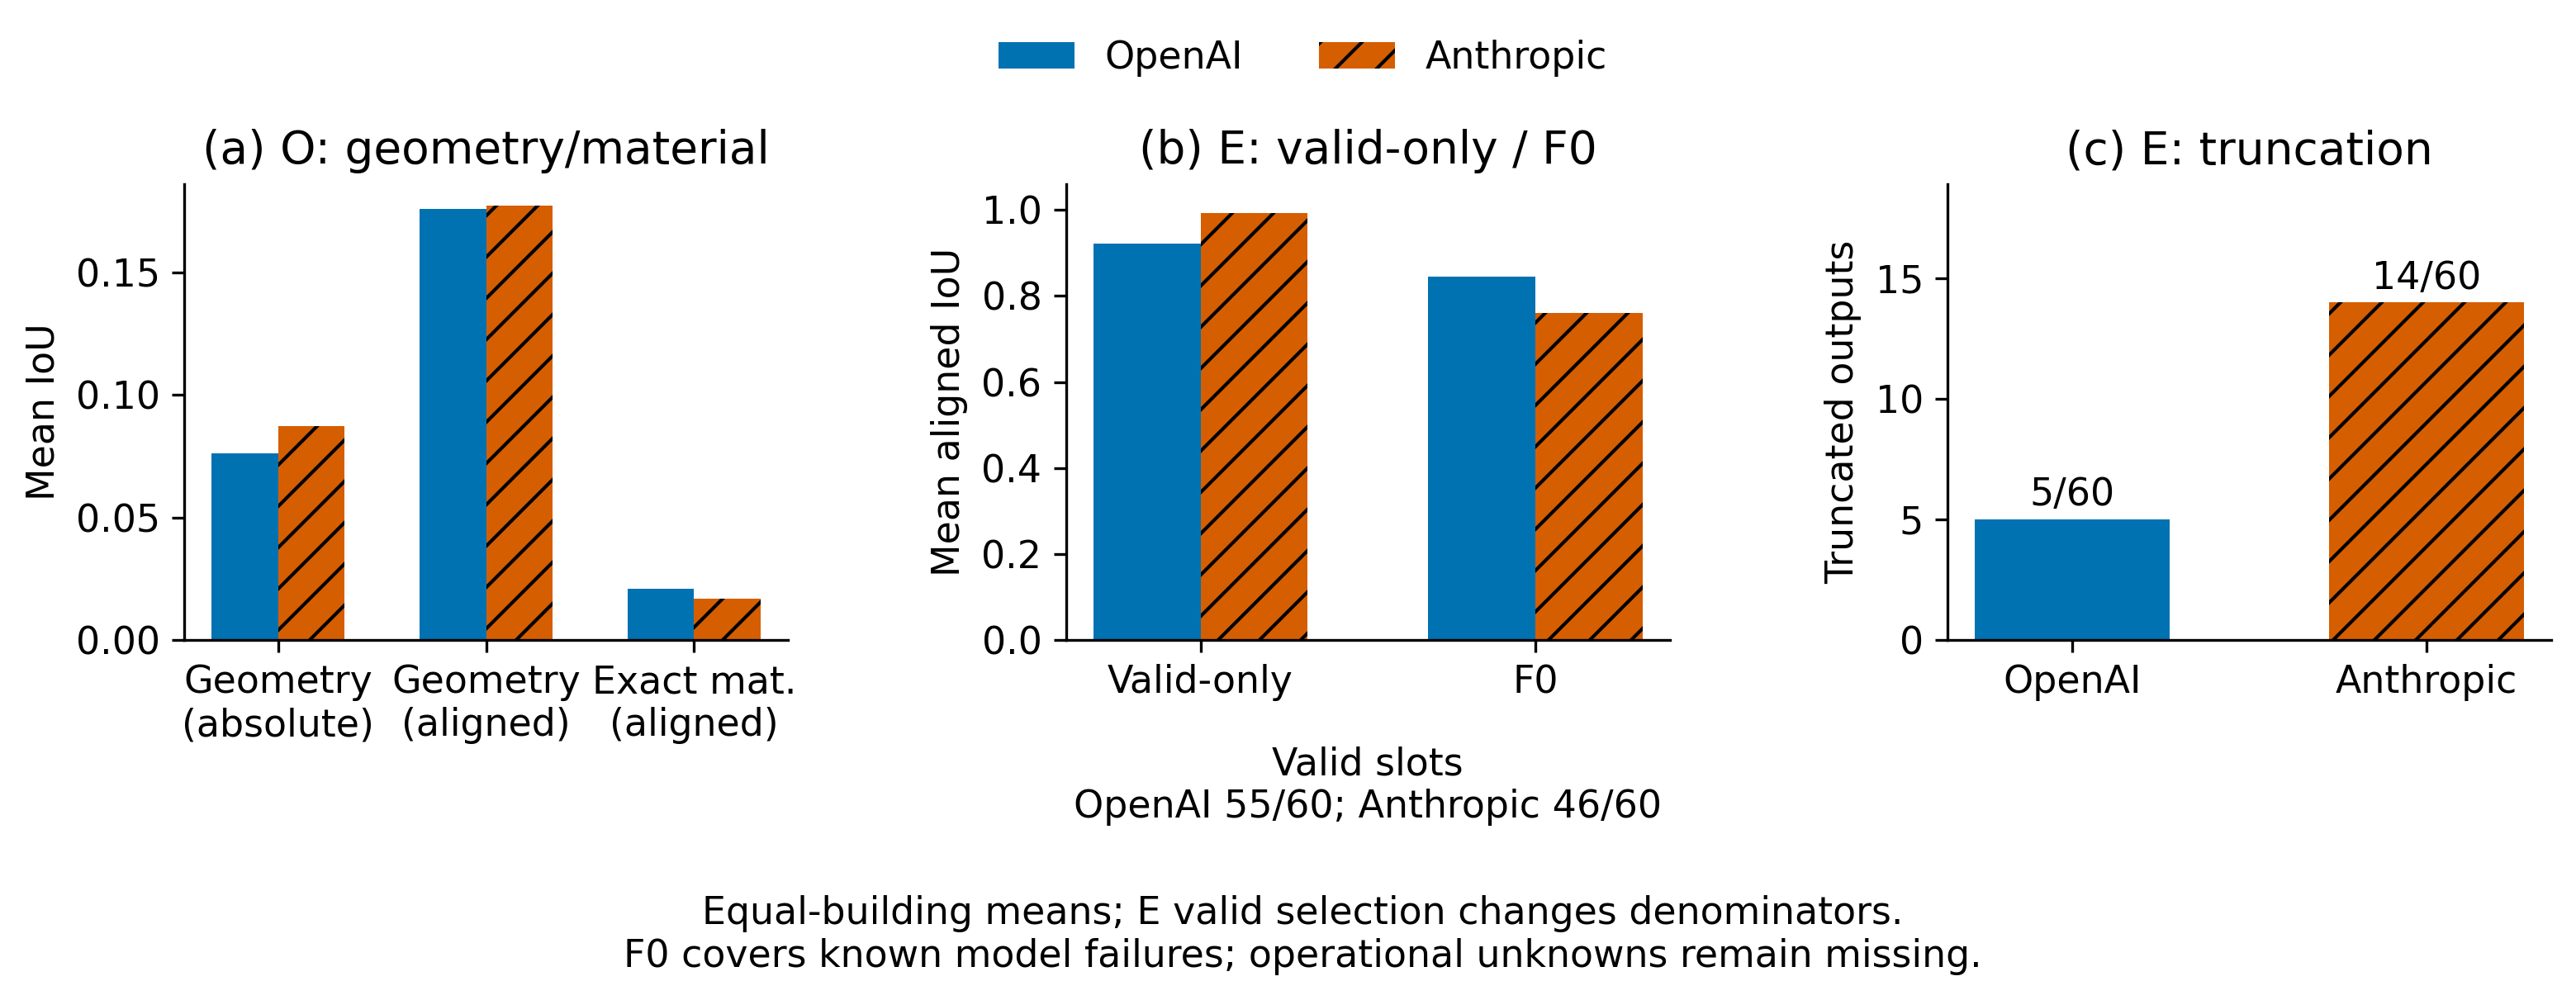
\includegraphics[width=\textwidth]{figure_main_errors.png}
\caption{Frozen Goal007 errors: (a) O absolute/aligned geometry and aligned exact-material-aware voxel IoU; (b) E valid-only and known-failure-zero aligned IoU; (c) E truncation. Means weight buildings equally, with valid selection changing denominators. F0 includes only identified completed model failures, never slot 942 HTTP 520. E valid-only values are conditional, not population upper bounds. No new inference is performed.}
\label{fig:goal008-main-errors}
\end{figure*}
\begin{figure*}[t]
\centering
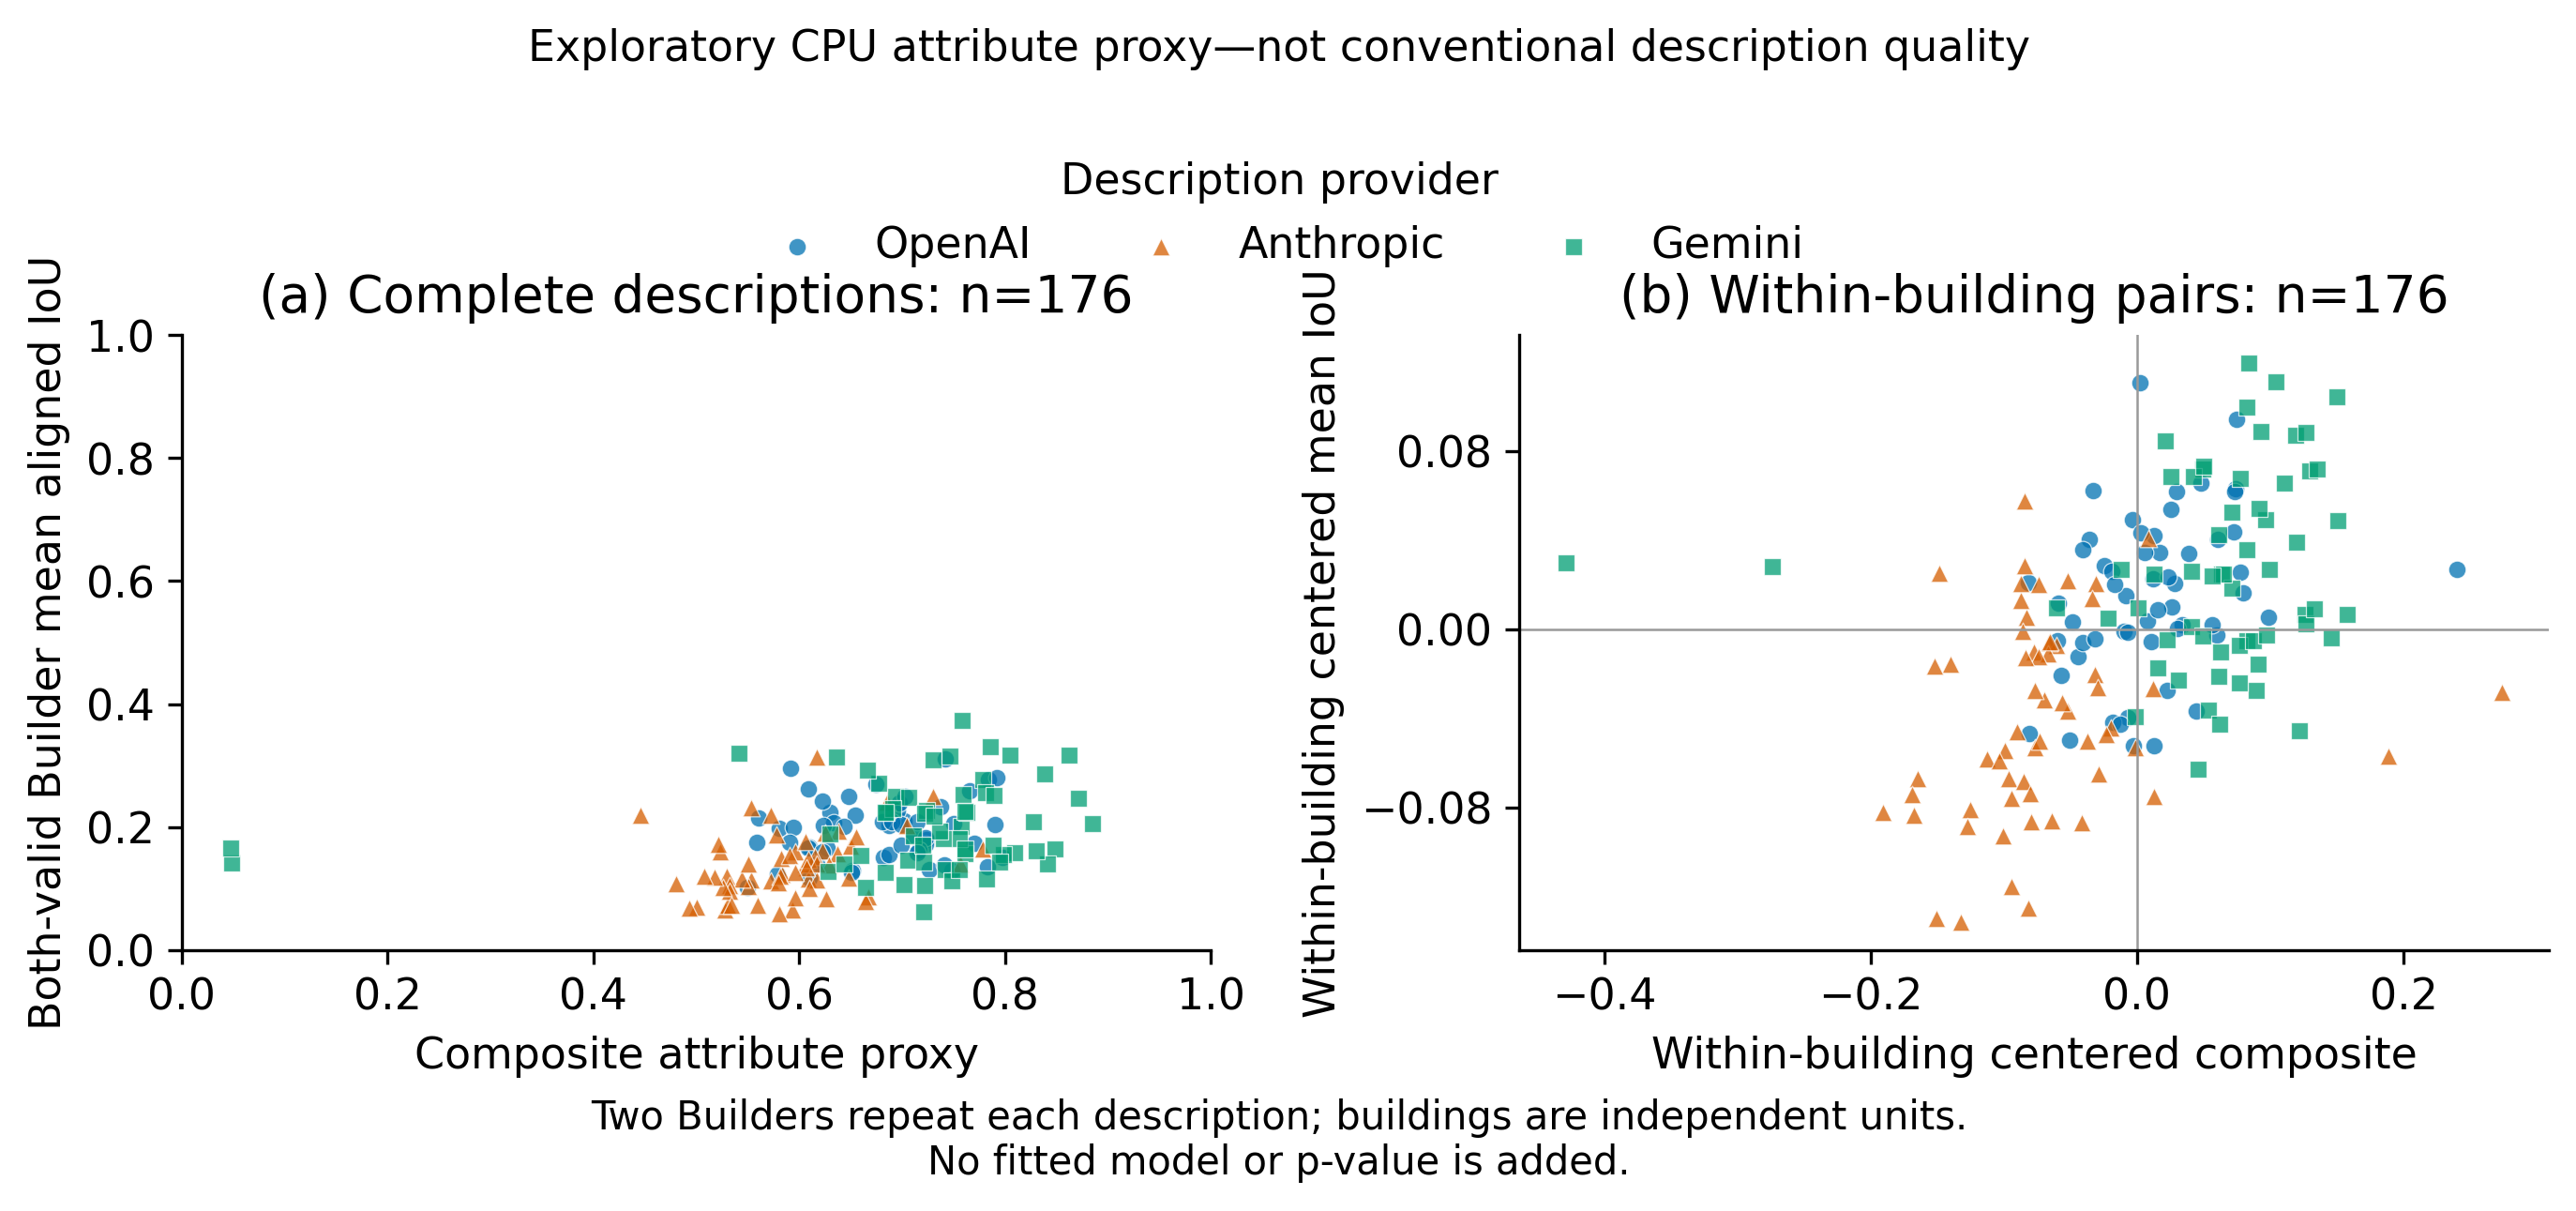
\includegraphics[width=\textwidth]{figure_proxy_scatter.png}
\caption{Exploratory CPU attribute proxy---not conventional description quality. Composite versus mean aligned IoU for descriptions with both Builders valid, and the same complete pairs centered within each building. Color and marker denote description provider. The two Builder outcomes are repeated observations, not independent descriptions; uncertainty in the separate tables resamples buildings. No fitted line or p-value is added. Shared GT and complete-case selection limit interpretation.}
\label{fig:goal008-proxy-scatter}
\end{figure*}

% Third body figure: three separately verified reconstruction-example rows.
\begin{figure*}[p]
\centering
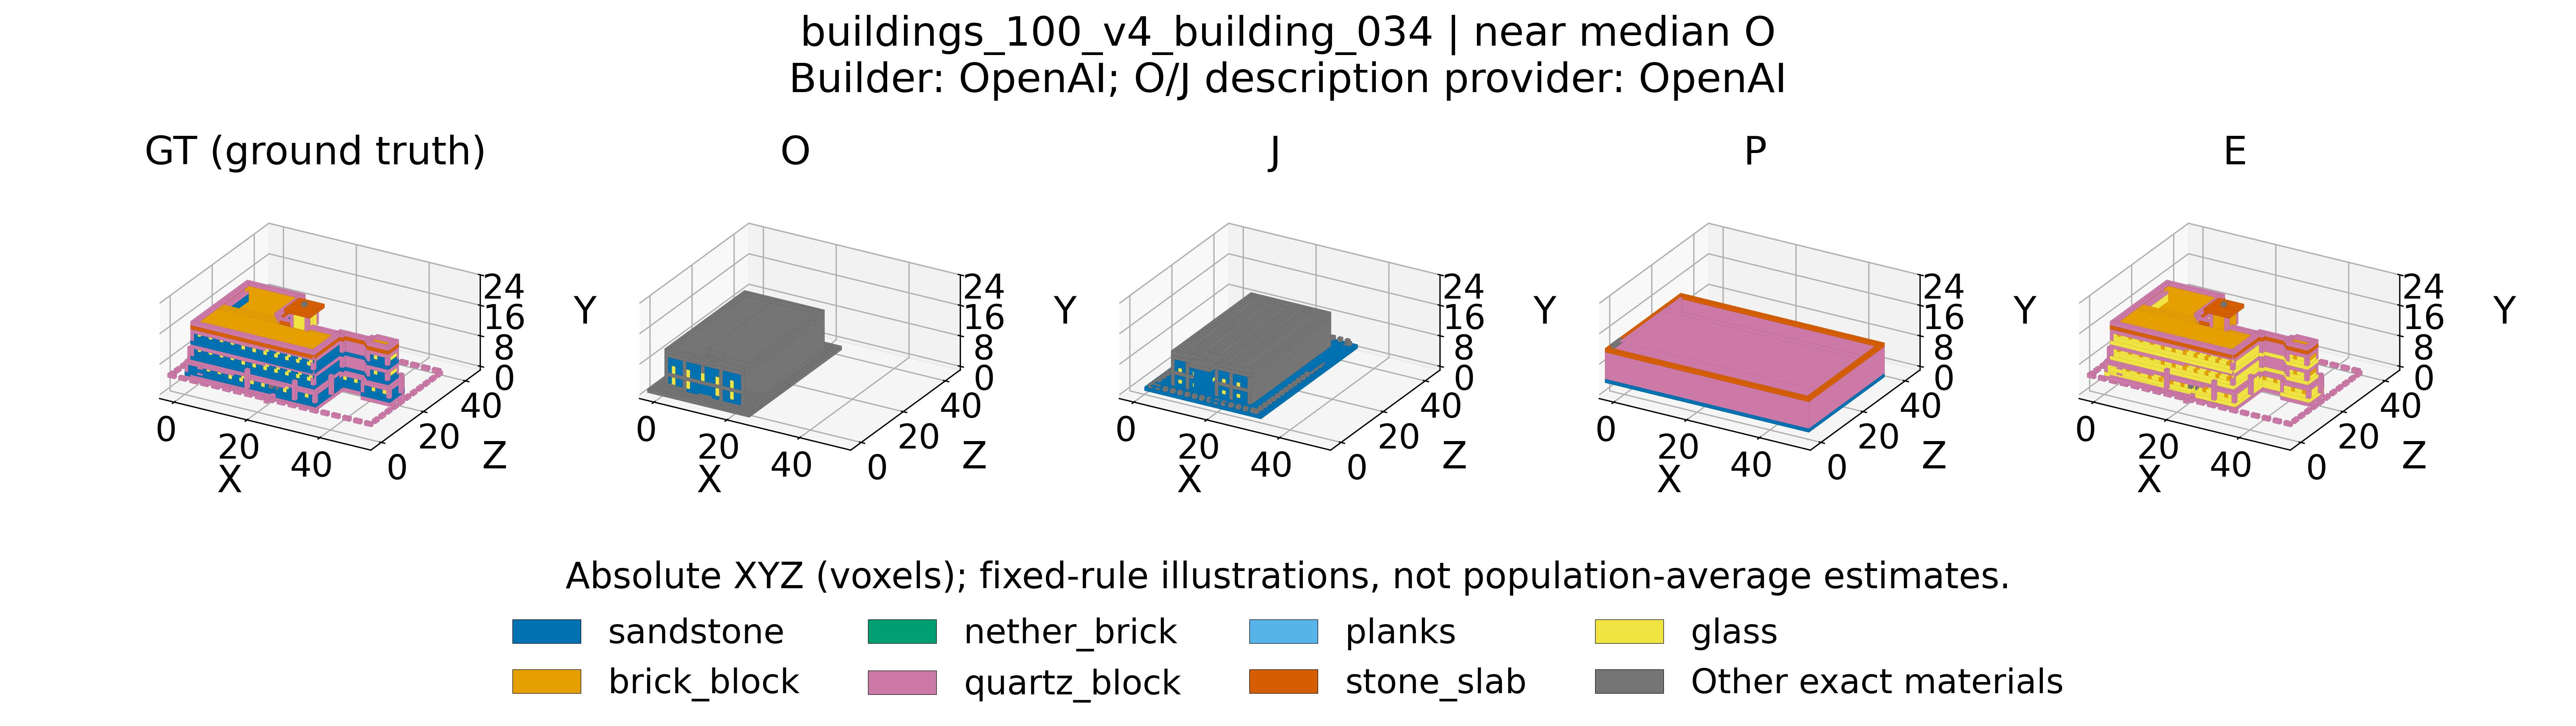
\includegraphics[width=\textwidth]{example_01.png}\\[2pt]
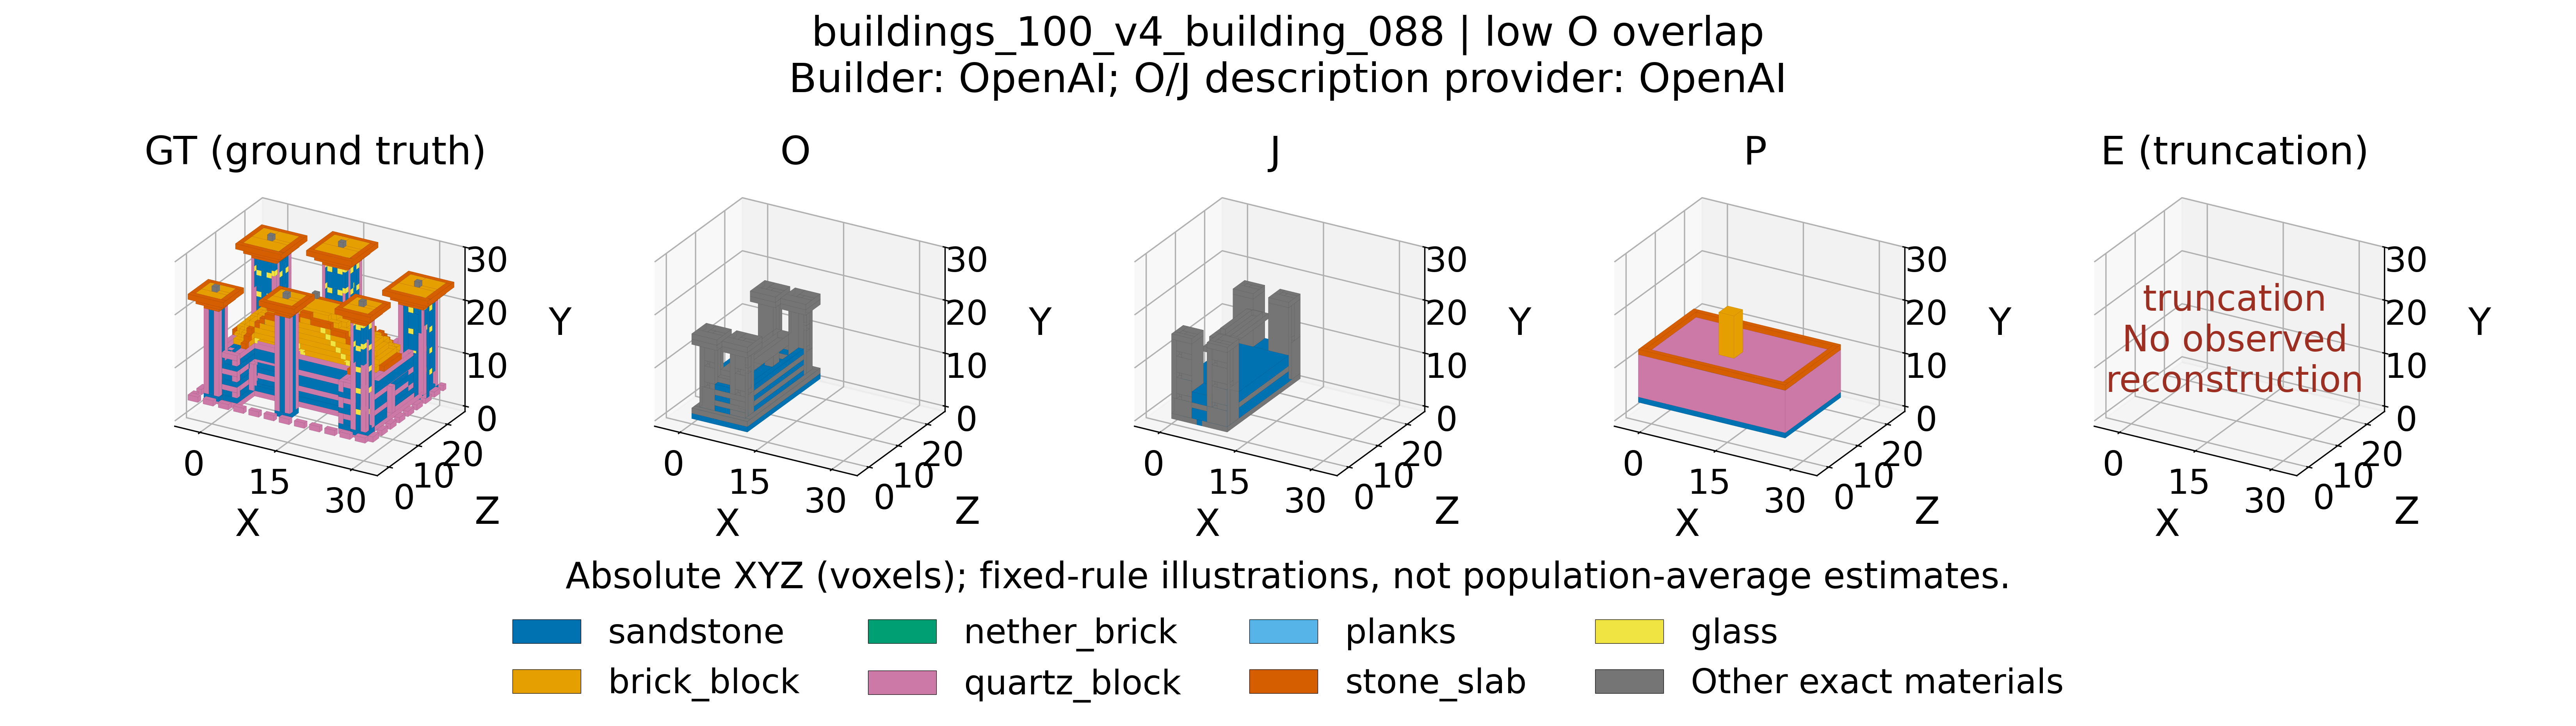
\includegraphics[width=\textwidth]{example_02.png}\\[2pt]
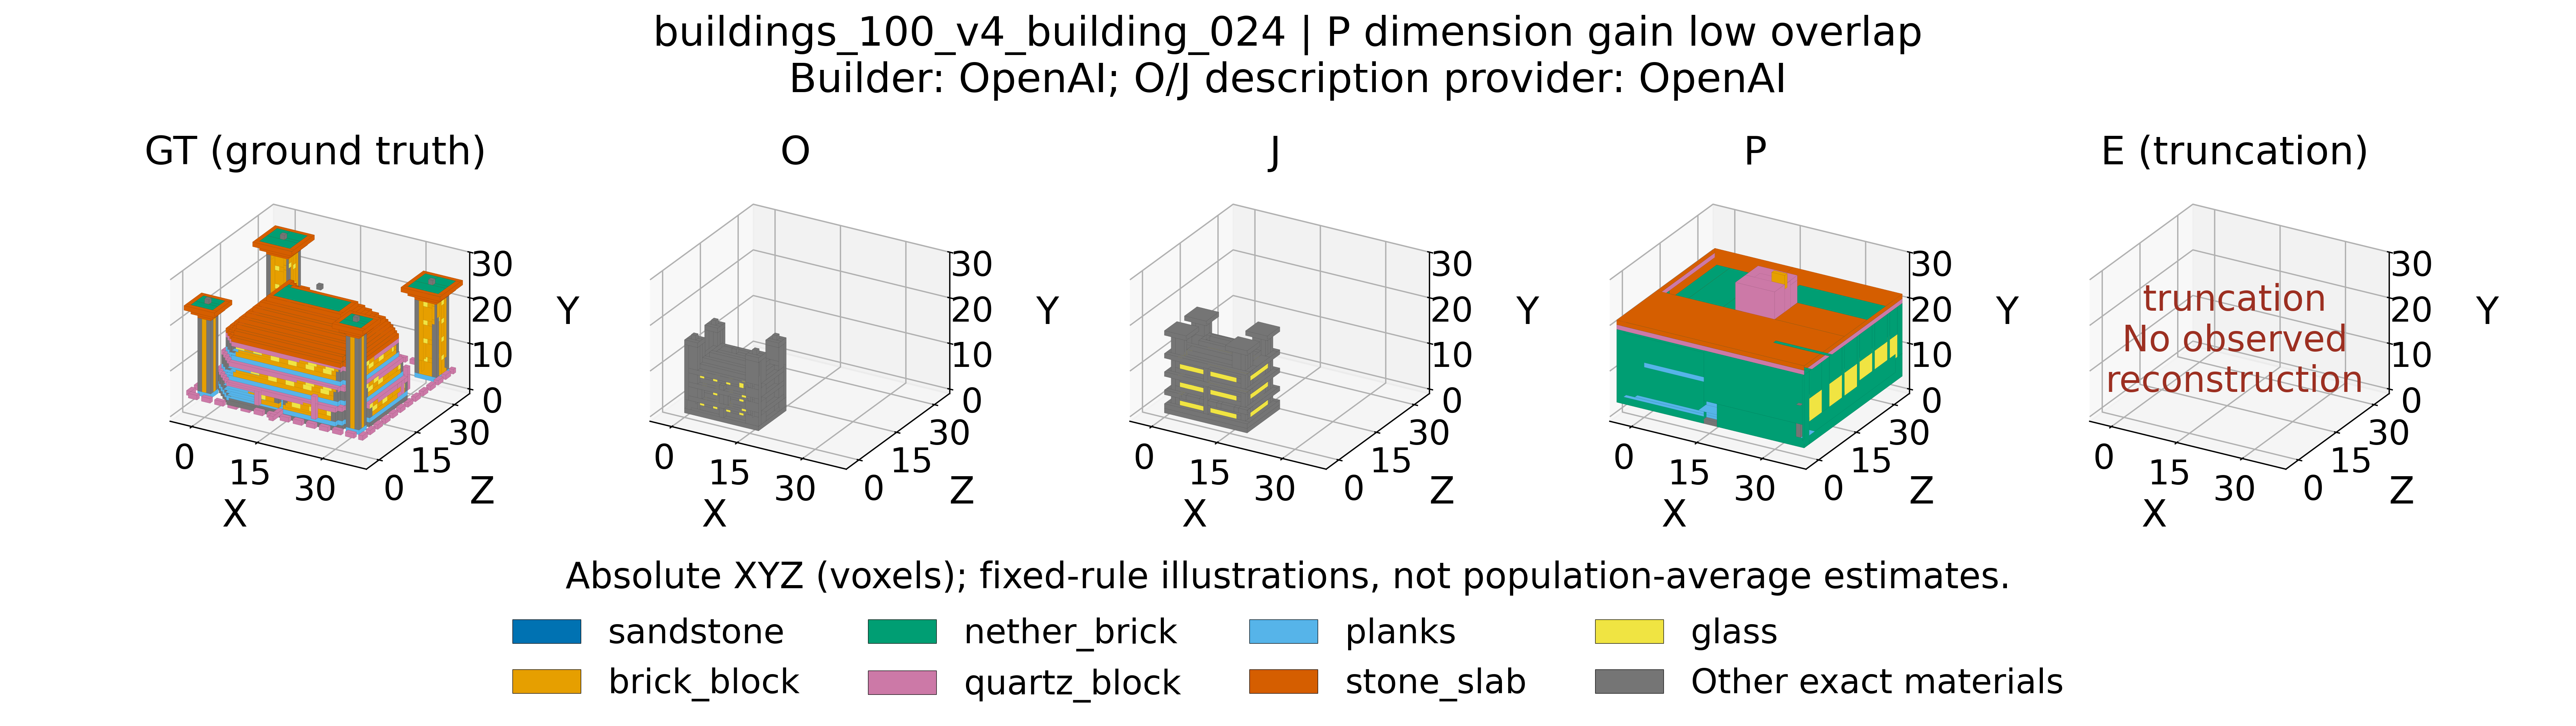
\includegraphics[width=\textwidth]{example_03.png}
\caption{Three distinct buildings selected by the fixed near-median O, low-O-overlap,
and P-dimension-gain with P IoU at most 0.20 rules, respectively.
All panels use unmodified absolute world coordinates, a common orthographic camera,
and identical axes and voxel scale within each row. The stored strict-aligned metrics
were used for selection only. O is the saved JSON-form visual description record;
J preserves that JSON tree; P/E supply partial/full GT information.
Failed E outputs remain explicitly marked, with no invented geometry.
Colors group the seven most frequent exact GT materials and other materials for display
only; exact identities and metrics remain in the source table.
These illustrative examples do not estimate population-average performance.
Source hashes, literal description excerpts, metrics and per-panel provenance appear in
the accompanying example table and manifest.}
\label{fig:goal008-reconstruction-examples}
\end{figure*}

